\documentclass[french]{beamer}
\usepackage{graphicx}
\usepackage{caption}

\usepackage[utf8]{inputenc}
\usepackage[T1]{fontenc}
\usepackage{lmodern}
\usepackage{amsmath, amssymb}

\usepackage{babel}


%CHOIX DU THEME et/ou DE SA COULEUR
% => essayer différents thèmes (en décommantant une des trois lignes suivantes)
%\usetheme{PaloAlto}
%\usetheme{Madrid}
%\usetheme{Copenhagen}
%\usetheme{CambridgeUS}

\usetheme{Hannover}

\useoutertheme[height=0pt,left]{sidebar}
\usecolortheme{beaver}
\setbeamercolor*{titlelike}{parent=structure}
\useinnertheme{circles}
\setbeamertemplate{frametitle}[default][right]



% => il est possible, pour un thème donné, de modifier seulement la couleur
%\usecolortheme{crane}
%\usecolortheme{seahorse}

%\useoutertheme[left]{sidebar}


%Pour le TITLEPAGE
\title{Analyse en Ondelettes}
\subtitle{Projet mathématiques-informatique}
\author[Rouyer, Gervais, Boulahia ]{ Chloé Rouyer, Pierre Gervais,  Souhaib Boulahia}
\date{\today}
\institute{Université Paris Diderot}


\begin{document}

\begin{frame}
	\titlepage
\end{frame}


\begin{frame}{Introduction}
	
	\begin{figure}[h]
		\centering
		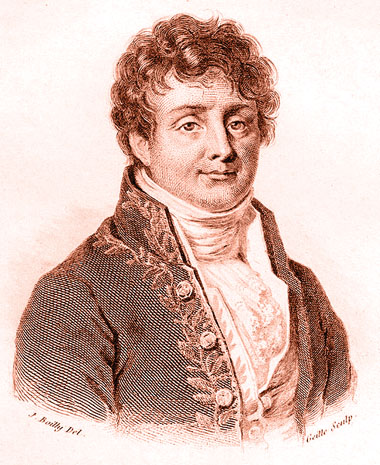
\includegraphics[width=100pt]{Fourier.jpg}
		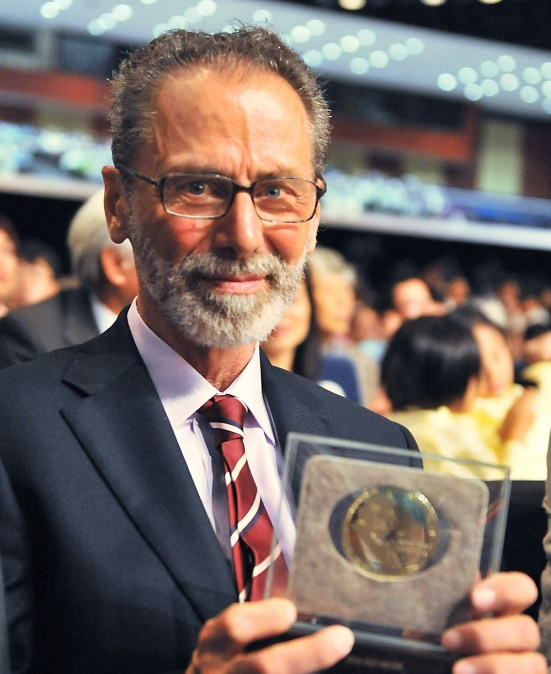
\includegraphics[width=100pt]{Meyer.jpg}
		\caption*{Joseph Fourier (1768 -1830) et Yves Meyer (1939- )}
	\end{figure}
	
\end{frame}

\begin{frame}{Sommaire}
	\tableofcontents
\end{frame}

\section{Outils}

\subsection{Analyse de Hilbert}
\begin{frame}{Analyse de Hilbert}
	
	
	
	
\end{frame}

\subsection{Espaces de Lebesgue}

\begin{frame}{Espaces de Lebesgue}

\end{frame}


\end{document}
















\begin{frame}
	Un \textbf<2,3>{texte} en gras. 
	\visible<3>{Un texte visible sur la 3\ieme{} couche}
\end{frame}

\begin{frame}{Titre (facultatif)} 
	\framesubtitle{Sous titre (facultatif aussi)}
	\begin{block}{Remarque}
		Un bloc
	\end{block}
	
	\begin{alertblock}{Proposition}
		Un bloc alerte
	\end{alertblock}
	
	\begin{exampleblock}<2>{Exemple}
		Un bloc exemple qui est visible sur la 2\ieme{} couche : $f(x)=2x$.
	\end{exampleblock}
\end{frame}

\section{Section 2}
\begin{frame}{La section 2 commence}
	\begin{itemize}
		\item<1-> On peut cliquer sur les titres de la barre de gauche pour naviguer dans les sections du pdf (essayez !).
		\item<2-> On peut changer le ``look'' du beamer, en changeant de thème. Retournez dans le fichier source et compilez avec les autres thèmes proposés (il existe énormément de thèmes; seuls trois sont proposés dans le source).
	\end{itemize}
	
\end{frame}